\normalsize
\subsection{Gravity Current Simulations - Staggered Grid}
\label{chapter:NumericalTest-Staggered}

The gravity current simulations are performed with two-dimensional staggered grid of different resolutions, $NX \times NZ = 140 \times 60$, $280 \times 120$, and $560 \times 240$. The time integration uses a four-stage, order-three explicit strong-stability-preserving Runge-Kutta method \cite{Ruuth2004} with the time step $\Delta t = 0.00375 (sec)$. It can be seen that the plots of $280 \times 120$ and $560 \times 240$ are fairly similar, implying that in this case, the simulation result with resolution of $280 \times 120$ is capable of describing that with higher resolutions.
\begin{figure}[htbp]
  \begin{center}
\subfigure[$NX \times NZ = 140 \times 60$] % caption for subfigure a
{
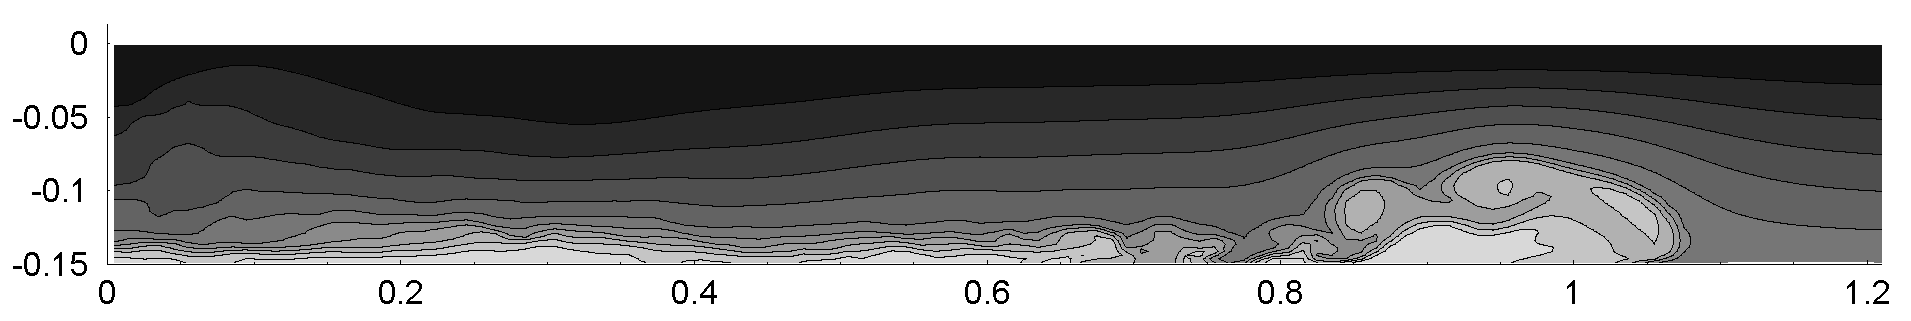
\includegraphics[width=5.2in]{../figures/Staggered/Fig9case/060518c-SSPRK35-dt-00375-140-60/08.png}
}
\subfigure[$NX \times NZ = 280 \times 120$] % caption for subfigure b
{
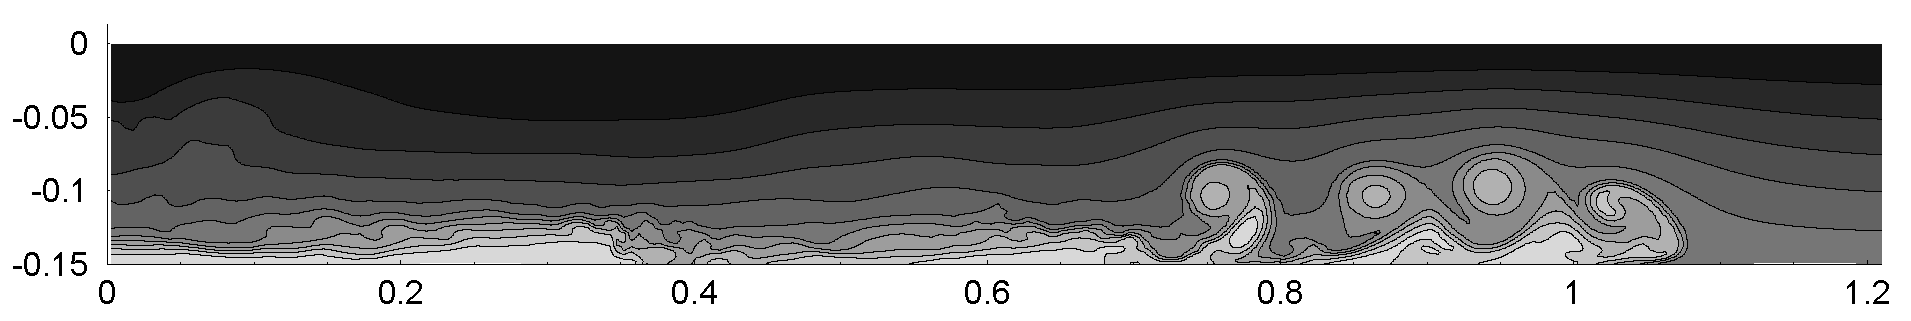
\includegraphics[width=5.2in]{../figures/Staggered/Fig9case/060518c-SSPRK35-dt-00375-280-120/08.png}
}
\subfigure[$NX \times NZ = 560 \times 240$] % caption for subfigure b
{
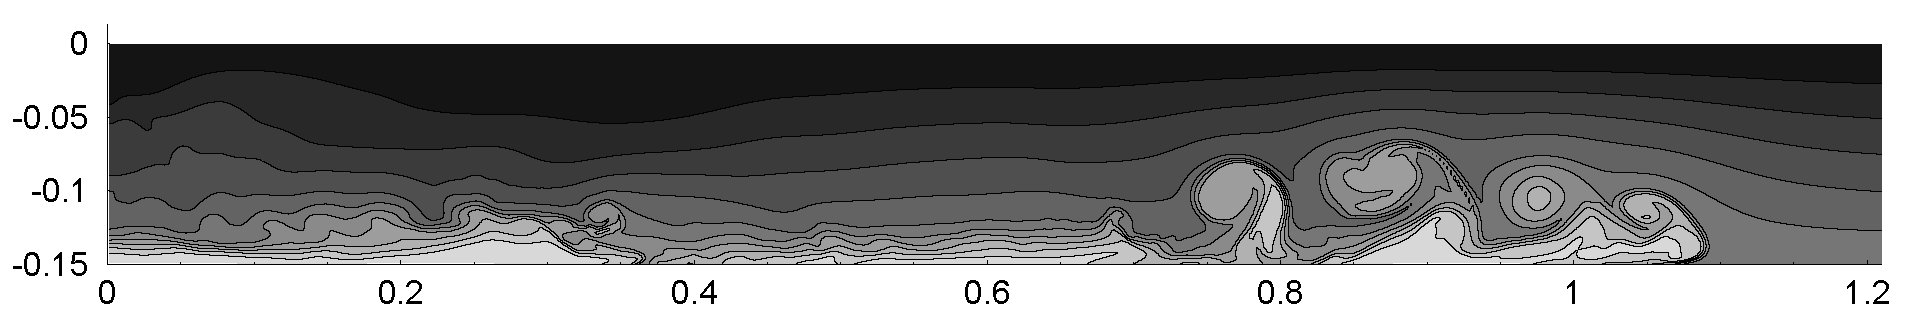
\includegraphics[width=5.2in]{../figures/Staggered/Fig9case/060526a-560-240-00375-VE-6/08.png}
}
\caption{Gravity current simulation plots at $t=6.3 (sec)$ with staggered grid and Strong-Stability- Preserving Runge-Kutta time integration scheme.}
  \end{center}
\end{figure}

\cp

\normalsize
\subsection{Gravity Current Simulations - Time Integration Scheme}

In this section the simulations are run with the same staggered grid discretization of $NX \times NZ = 280 \times 120$ but with different time integration schemes, viz, Euler, RK4, and SSPRK35. The following figure shows that these different time integration schemes generate similar results, while the SSPRK scheme can stably finish the simulation with fewer iterations.
\begin{figure}[htbp]
  \begin{center}
\subfigure[Time integration with forward Euler method and $\Delta t = 0.000234375$] % caption for subfigure a
{
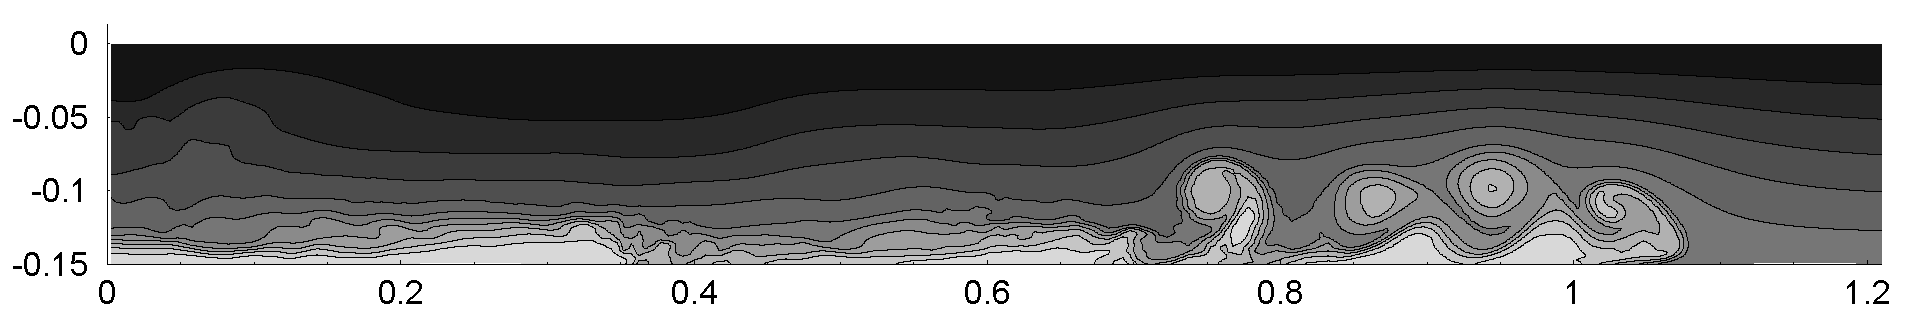
\includegraphics[width=5.2in]{../figures/Staggered/Fig9case/060519b-Euler-dt-000234375-280-120/08.png}
}
\subfigure[Time integration with Rung-Kutta 4th order method and $\Delta t = 0.0009375$] % caption for subfigure b
{
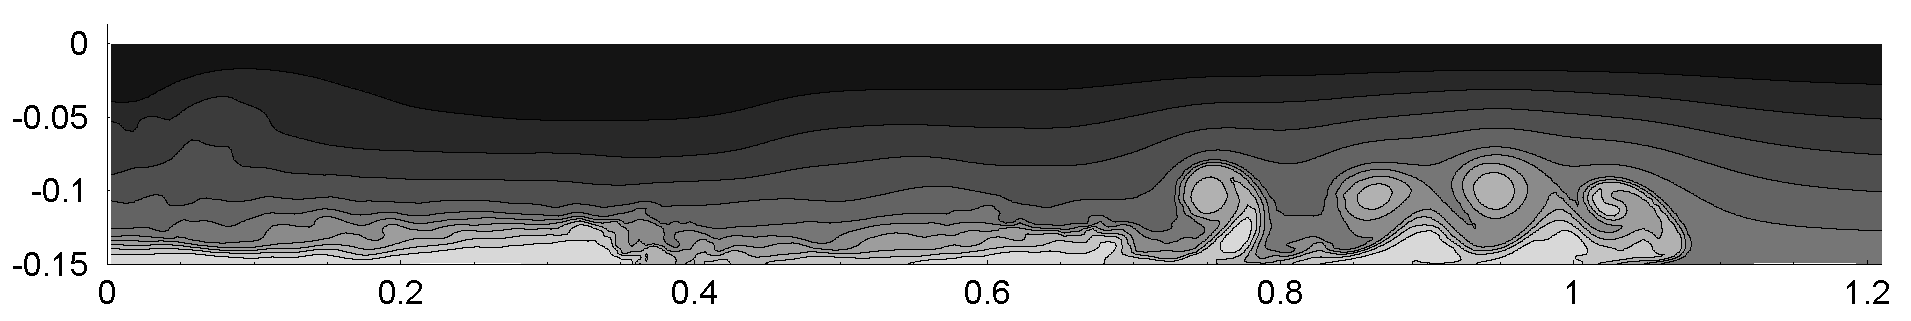
\includegraphics[width=5.2in]{../figures/Staggered/Fig9case/060518c-RK4-dt-0009375-280-120/08.png}
}
\subfigure[Time integration with 4-step order-3 Strong-Stability-Preserving Runge-Kutta method and $\Delta t = 0.001875$] % caption for subfigure b
{
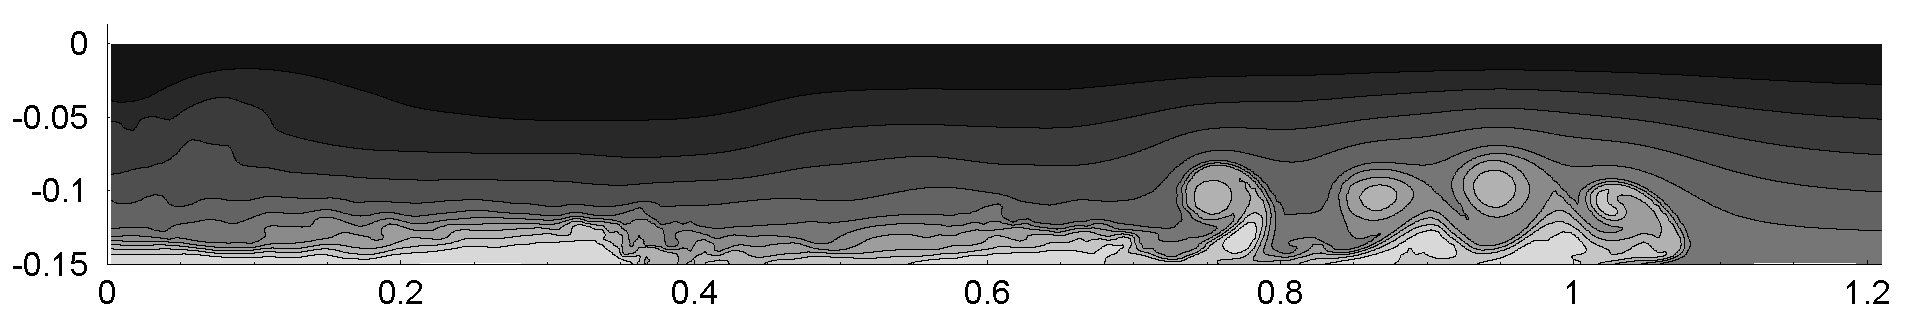
\includegraphics[width=5.2in]{../figures/Staggered/Fig9case/060518c-SSPRK35-dt-001875-280-120/08.png}
}
\subfigure[Time integration with 4-step order-3 Strong-Stability-Preserving Runge-Kutta method and $\Delta t = 0.0075$] % caption for subfigure b
{
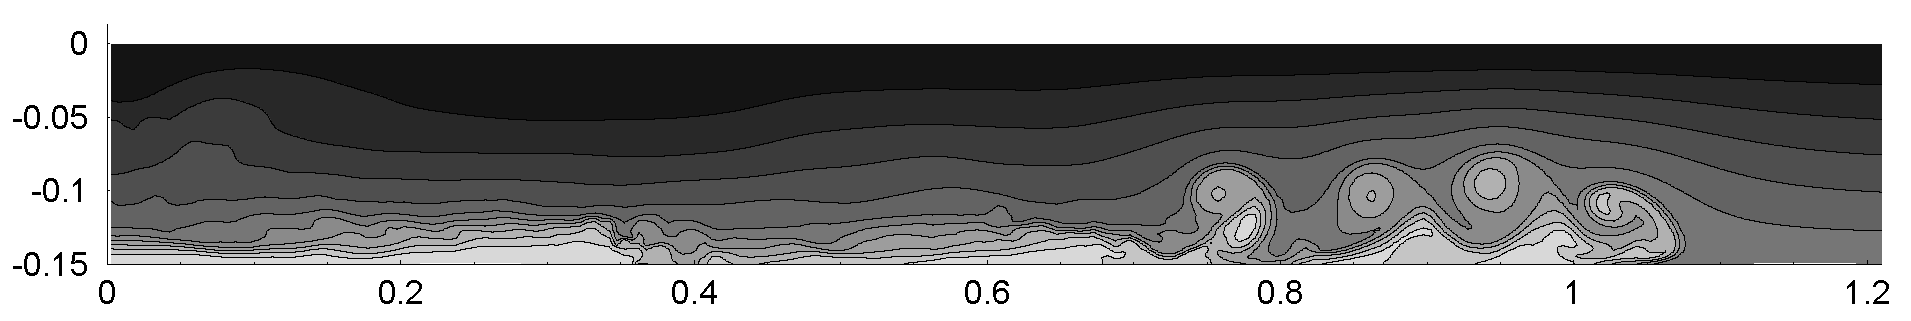
\includegraphics[width=5.2in]{../figures/Staggered/Fig9case/060518c-SSPRK35-dt-0075-280-120/08.png}
}
\caption{Gravity current simulation plots at $t=6.3 (sec)$ with staggered grid and different time integration scheme.}
  \end{center}
\end{figure}

\cp 